\begin{cpa}
 \chapter{Thermodynamics of proton hydration and the electrochemical surface potential}
 \hyperlink{toc}{Return to TOC}
  \section{\label{ch5:sec0:level1}Preface}
  Much of the text presented here has been adapted from the following publications,
  
  \vspace{12pt}
  \noindent \emph{Travis P.~Pollard, Thomas L.~Beck, Quasichemical analysis of the cluster-pair approximation for the thermodynamics of proton hydration, 
  J. Chem. Phys. \textbf{140} (22) 2014.}

  \noindent \emph{Travis P.~Pollard, Thomas L.~Beck, The thermodynamics of proton hydration and the electrochemical surface potential of water, J. Chem. Phys. 
  \textbf{141} (18C512) 2014.}
  \vspace{12pt}
  
  These articles summarize the findings of my computational analysis of the cluster-pair approximation (CPA) for the determination of single-ion free energies and
  enthalpies from the extrapolation of cluster data to the bulk. The CPA expression of these quantities for the proton includes an interfacial potential 
  contribution by definition. It is shown, however, that the CPA involves an extra-thermodynamic assumption that does not guarantee uniform convergence to a bulk 
  free energy or enthalpy value with increasing cluster size. I use computational modeling to examine the size-dependence of the differences in the hydration enthalpies 
  for the Na\sur{+}/F\sur{-} ion pair in water clusters of size \emph{n} = 1, 2, 3, \dots, 200 (not perfectly sequential, there are some breaks). A sizable shift from
  the accepted cluster-pair approximation value is found for the proton hydration enthalpy for cluster sizes just beyond the limits used in the CPA. The shifts arise 
  from a combination of sequential hydration and interfacial potential effects and converges at large \emph{n} to a value of -0.4 V to -0.5 V depending on the
  temperature derivative of the interfacial potential being used. The -0.4 V result is argued to be preferable and assumes the temperature derivative to be close to
  0.~cal/mol-K-\emph{e}. In response to concerns raised that the 2$^{nd}$ order M$\text{\o}$ller-Plesset (MP2) energy overestimates the dispersion energy in 
  F\sur{-}/water clusters leading to the shift\cite{herbert2014personal}, I have included previously unpublished evaluations of the enthalpy differences using the 
  `gold standard' CCSD(T) method. Though the cluster size is severely limited, the beginnings of the shift are shown to be preserved.
  
  This section addresses three of the questions I posed in Chapter \ref{ch1:sec1:level4},
   
   \begin{itemize}
       \item Do chemical interfaces contribute to single-ion thermodynamics? 
       \item If so, what is the contribution?
       \item How can we compare our simulation results to experiment?
   \end{itemize}
  
  \section{\label{ch5:sec1:level1}The cluster pair approximation}
  The cluster-pair approximation\cite{coe1998cpa1} (CPA) is widely viewed as the most accurate approach for determining the hydration free energy of the 
  proton\cite{camaioni2005stdstcorr,kelly2006cpa} Given the hydration free energy of one ion, all other single-ion free energies can be obtained from bulk 
  thermodynamic data\cite{conway1978evaluation,marcus1985book}. The CPA approach utilizes ion-water cluster data and bulk conventional ion hydration free energies 
  (referenced to the proton), along with an insightful analysis, to infer the proton hydration enthalpy and free energy. Recently, the issue has been
  raised as to whether the CPA may involve an extra-thermodynamic assumption that could result in proton values that deviate from those predicted based
  on small-cluster data\cite{donald2010expand_cpa,hunenberger2011sp,vlcek2013cpa,vlcek2016cpareview}. This deviation is predicted to result from two
  parts: 1) hydration effects and 2) the net potential of water $\phi\sous{np}$. At large \emph{n} it is expected that the shift be comprised of 
  $\phi\sous{np}$ alone.

  The excess chemical potential can be written as\cite{aquaincognita2014} 
  
  \begin{equation} 
    \mu_X^{ex} = \mu_{X,b}^{ex} + q\phi_{np}
    \label{eq:echemmu}
  \end{equation}

  \noindent where $\mu_{X,b}^{ex}$ is the bulk hydration free energy (that includes all interactions of the ion with water except for the net potential 
  contribution), see discussion in Chapter \ref{ch1:sec4:level1}. $\mu_{X,b}^{ex}$ is also called the \emph{intrinsic} free energy\cite{hunenberger2011sp}
  and $\mu_X^{ex}$ the \emph{real} free energy. Similar nomenclature is extended to the hydration enthalpy which is
  
  \begin{equation}
    h_X^{ex} = h_{X,b}^{ex} + q\phi_{np} - qT\left(\frac{\partial \phi_{np}}{\partial T}\right)_P
    \label{eq:echemh}
  \end{equation}

  \noindent and the hydration entropy\cite{lynden1997hydrophobic} is

  \begin{equation}
    s_X^{ex} = s_{X,b}^{ex} - q\left(\frac{\partial \phi_{np}}{\partial T}\right)_P.
    \label{eq:echems}
  \end{equation}

  \noindent In these papers, standard states of 1 M concentration in both the vapor and liquid phases are used so that the free energies and entropies 
  reflect excess quantities that do not include superfluous volume changes. The experimental value for the temperature derivative is taken as -9.9 
  cal/mol-K-\emph{e}\cite{randles1977structure}, though there is evidence this value is much too negative\cite{donald2010expand_cpa,vlcek2013cpa}.

  To understand the origins of the CPA, consider the exact QCT expression for the ion excess chemical potential from Ref. \cite{asthagiri2010ion}
  
  \begin{equation}
    \mu_X^{ex} = -kT \ln [K_{X,n}^{(0)} \rho_W^n] + kT \ln p_X(n) + \mu^{ex}_{XW_n} - n\mu^{ex}_W  
    \label{eq:qctcpl}
  \end{equation}

  \noindent where $K_{X,n}^{(0)}$ is the equilibrium constant for the formation of the $XW_n$ cluster in the gas phase, $\rho_W$ is the bulk density of 
  water, $p_X(n)$ is the probability of observing \emph{n} waters complexed with the ion in bulk water, $\mu^{ex}_{XW_n}$ is the free energy to insert the 
  cluster into bulk water, and $\mu^{ex}_W$ is the free energy to insert one water molecule into bulk water.

  Collecting all terms but the free energy to hydrate the cluster into a single term $\mu^{ex}_{X,n}$
  
  \begin{equation}
    \mu_X^{ex} =  \mu^{ex}_{X,n} + \mu^{ex}_{XW_n}  
    \label{eq:qctcpa}
  \end{equation}

  \noindent where
  
  \begin{equation}
    \mu^{ex}_{X,n} = -kT \ln K_{X,n}^{(0)} + kT \ln p_X(n) - n \left[ kT \ln \rho_W  + \mu^{ex}_W \right] 
    \label{eq:qctcpaxn}
  \end{equation}

  \noindent The first two terms on the right side of Eq. \ref{eq:qctcpaxn} are ion specific, while the last term involves properties of bulk water.
  The cluster experimental data employed in the CPA\cite{coe1998cpa1} involves the temperature dependence of $K_{X,n}^{(0)}$ for small clusters 
  \emph{n} = 1--6. The CPA relies on differences of free energy and enthalpy terms for positive/negative ion pairs. Then all terms in $\mu^{ex}_{X,n}$ 
  except $K_{X,n}^{(0)}$ cancel when taking the differences (for large \emph{n}, the term involving $p(n)$ should also cancel nearly exactly).

  The terms in Eq. \ref{eq:qctcpa} correspond to a 2-step process for analyzing the hydration free energy: formation of the ion-water cluster 
  followed by insertion of the cluster into bulk water. It is clear on physical grounds that cation/anion differences of $\mu^{ex}_{XW_n}$
  approach zero as the cluster size approaches infinity, since this is the free energy to insert a large ion/water cluster into bulk water, and on
  average the ion is thus shielded from the surrounding bulk water. 

  The input data for the CPA\cite{coe1998cpa1} includes differences of bulk conventional free energies and cluster formation free energies for cation/anion 
  pairs; the cluster free energies are available for a range of ions with \emph{n} = 1--6 clustered waters. These data have been assembled from mass 
  spectrometric analyses on ion/water clusters with size discrimination based on collision energy\cite{wheeler2015hydration} or other means and theoretical 
  calculations\cite{coe1998cpa1,coe2001cpa2,coe2002cpa3,donald2010expand_cpa,kelly2006cpa}.
  
  The bulk conventional free energies are defined as
  
  \begin{equation}
    \mu_N^{ex,con} =  \mu^{ex}_{N} + \mu^{ex}_{\mathrm{H}^+} = \mu^{ex}_{N,b} + \mu^{ex}_{\mathrm{H}^+,b}
    \label{eq:con1}
  \end{equation}

  \noindent for a negatively charged ion and

  \begin{equation}
    \mu_P^{ex,con} =  \mu^{ex}_{P} - \mu^{ex}_{\mathrm{H}^+} = \mu^{ex}_{P,b} - \mu^{ex}_{\mathrm{H}^+,b}
    \label{eq:con2}
  \end{equation}
  
  \noindent for a positively charged one, where the bulk free energies are $\mu^{ex}_{X,b} = \mu^{ex}_{X} - q\phi_{np}$. The conventional free 
  energies can be obtained from bulk thermodynamic data, and it is apparent that the net potential does not appear explicitly in Eqns. \ref{eq:con1} 
  and \ref{eq:con2} due to the cancellation between the ion and proton terms. The conventional free energy scale is set relative to the proton,
  just as the electrochemical scale (the standard hydrogen electrode has a potential of 0. V, when the \emph{real} potential is estimated at 
  -4.44 $\pm$ 0.02 V\cite{trasatti1986absolute}).

  The CPA is an analysis method that leads to an estimation of the proton hydration free energy, enthalpy, and entropy. For brevity, I'll review
  only the free energy `path.' First, consider the free energy difference between a cation ($P$) and anion ($N$), defined for example as
  
  \begin{equation}
    \Delta \mu_X^{ex,con} =  \mu^{ex,con}_{N} - \mu^{ex,con}_{P}  
    \label{eq:cpadiff}
  \end{equation}

  \noindent so the change refers to the $P \rightarrow N$ transition for a given ion pair. Combining this expression with those above in Eqns.
  \ref{eq:con1} and \ref{eq:con2} results in the following relationships

  \begin{equation}
    \frac{1}{2} \Delta \mu_{X}^{ex,con} - \frac{1}{2} \Delta \mu_{X}^{ex} = \mu^{ex}_{\mathrm{H}^+}
    \label{eq:cpa1}
  \end{equation}

  \noindent and
  
  \begin{equation}
    \frac{1}{2} \Delta \mu_{XW_n}^{ex,con} -  \frac{1}{2} \Delta \mu_{XW_n}^{ex} = \mu^{ex}_{\mathrm{H}^+}.
    \label{eq:cpa2}
  \end{equation}

  \noindent It is also true that 
  
  \begin{equation}
    \frac{1}{2} \Delta \mu_{X}^{ex,con} - \frac{1}{2} \Delta \mu_{X,b}^{ex} + \phi_{np} = \mu^{ex}_{\mathrm{H}^+}
    \label{eq:cpa1bulk-1}
  \end{equation}
  
  \noindent and 

  \begin{equation}
    \frac{1}{2} \Delta \mu_{X}^{ex,con} - \frac{1}{2} \Delta \mu_{X,b}^{ex} = \mu^{ex}_{\mathrm{H}^+,b}.
    \label{eq:cpa1bulk}
  \end{equation}

  \noindent Since $\Delta \mu_{X}^{ex}$ and $\Delta \mu_{XW_n}^{ex}$ are not available from experiment, the CPA makes an assumption to deal with 
  these terms. 

  $\Delta \mu_{X}^{ex,con}/2$ contains no explicit net potential contribution; it is clear from Eq. \ref{eq:qctcpa}, however, that $\Delta 
  \mu_{XW_n}^{ex,con}/2$ can develop an explicit net potential contribution for large \emph{n} due to the cluster term (since $\Delta 
  \mu^{ex,con}_{X} = \Delta \mu^{ex}_{X,n} + \Delta\mu^{ex,con}_{XW_n}$). It is also clear from Eq. \ref{eq:cpa2} that, in the limit of large 
  \emph{n}, $\Delta \mu_{XW_n}^{ex,con}/2 = \mu^{ex}_{\mathrm{H}^+}$.

  Eq. \ref{eq:cpa1} can be rewritten as
  
  \begin{equation}
    \frac{1}{2} \Delta \mu_{X}^{ex,con} - \frac{1}{2} \left[ \mu_{N,n}^{ex}/c_{N,n} - \mu_{P,n}^{ex}/c_{P,n} \right] = \mu^{ex}_{\mathrm{H}^+}
    \label{eq:cpa3}
  \end{equation}
  
  \noindent where $c_{N,n} = \mu_{N,n}^{ex}/\mu_{N}^{ex}$ and $c_{P,n} = \mu_{P,n}^{ex}/\mu_{P}^{ex}$. The central assumption of the 
  CPA\cite{coe1998cpa1} is then to create a composite term for the chosen $N/P$ pair:

  \begin{equation}
    \bar{c}_{X,n} = \frac{\mu_{N,n}^{ex} + \mu_{P,n}^{ex}}{\mu_{N}^{ex} + \mu_{P}^{ex}}
    \label{eq:cpacomp}
  \end{equation}
  
  \noindent where now the quantities are experimentally available. Then

  \begin{equation}
    \frac{1}{2} \Delta \mu_{X}^{ex,con} - \frac{1}{2\bar{c}_{X,n}} \Delta \mu_{X,n}^{ex} \approx \mu^{ex}_{\mathrm{H}^+}
    \label{eq:cpafinal}
  \end{equation}
  
  \noindent Since the exact relation involves 
  
  \begin{equation} 
    \bar{c}_{X,n} (\mathrm{exact}) = \frac{\mu_{N,n}^{ex} - \mu_{P,n}^{ex}}{\mu_{N}^{ex} - \mu_{P}^{ex}} = \frac{\Delta \mu^{ex}_{X,n}}{\Delta \mu^{ex}_{X}}
    \label{eq:cpacompex}
  \end{equation}

  \noindent it is seen that the CPA involves an extra-thermodynamic assumption. In plain language, the assumption is that the differences
  in the pair solvation free energies for the small clusters should converge rapidly to the bulk limit and remain roughly constant to
  large \emph{n}. As mentioned previously, this is not necessarily the case\cite{donald2010expand_cpa,vlcek2013cpa,vlcek2016cpareview}.
 
  Assembling many differences for the alkali/halides and even broader ion sets, the results can be plotted as in Kelly, Cramer, and 
  Truhlar\cite{kelly2006cpa} (Figure 1 of Ref. \cite{kelly2006cpa}). The $y$ axis is 
  
  \begin{equation}
    y(n)=\frac{1}{2} \Delta \mu_{XW_n}^{ex,con}
    \label{eq:ydata}
  \end{equation}
  
  \noindent and the $x$ axis is 
  
  \begin{equation}
    x=\frac{1}{2} \Delta \mu_{X}^{ex,con}.
    \label{eq:xdata}
  \end{equation}

  \noindent The original CPA paper\cite{coe1998cpa1} uses a related expression but takes from Eq. \ref{eq:cpafinal} the y-axis as $\mu\sursous{ex}{H\sur{+}}$
  and the x-axis as $\Delta\mu_{X,n}^{ex}$. Refs. \cite{pollard2014cpa1} and \cite{pollard2014cpa2} use the former, but the latter is 
  important for understanding why I only needed to consider the Na\sur{+}/F\sur{-} ion pair for this study. A more exhaustive compilation
  of ion pairs would have produced identical results to within some error, but I'm using a trick here. The CPA figures when plotted with the
  latter pair of variables, produce the \emph{exact}, \emph{real} proton hydration free energy, enthalpy, or entropy when the difference 
  for an ion pair at a given \emph{n} is exactly zero. See Figure \ref{fig:coecpaexample} for reference. The differences in solvation free energies
  and enthalpies for the Na\sur{+}/F\sur{-} pair sit near zero for \emph{n} = 1--6, making them the \emph{ideal} pair of ions to explore the shift
  in the difference at larger \emph{n}. I also modify the F\sur{-} ion somewhat (discussed below) and this coincidentally further idealizes the pair.
  
\begin{figure}
 \begin{center}
  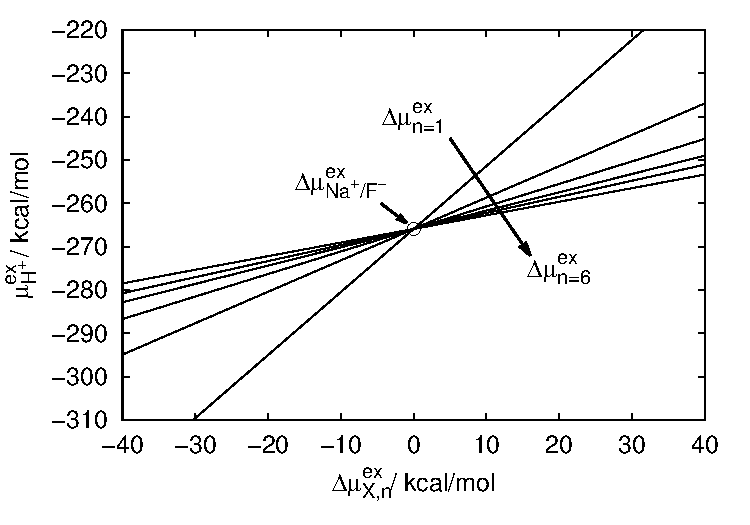
\includegraphics[width=0.98\linewidth]{images/cpa/cpa_example.pdf}
 \end{center}
\caption[Illustration of the cluster pair approximation for the proton solvation free energy]{Illustration of the cluster pair approximation for the
proton solvation free energy in the form described by Coe et al.\cite{coe1998cpa1}. Lines represent linear fits through all possible combinations of 
pairs and their differences (slopes taken directly from Ref. \cite{coe1998cpa1}). With increasing cluster size, the slope of the lines is reduced.
In the limit of \emph{n} $\rightarrow \infty$, the slope falls to zero defining $\mu\sursous{ex}{H\sur{+}}$. The lines also share an approximately 
common crossing point. This point sits very near the value of $\mu\sursous{ex}{H^{+}}$ even for \emph{n} = 1. Remarkable, really. The ion pair 
Na\sur{+} and F\sur{-} also sit very near the crossing point for \emph{n} = 1--6. By modeling the Na\sur{+} to F\sur{-} transition in 
$\mu\sursous{ex}{X,n}$ or other properties as a surrogate for the crossing point, I can test my prediction that the point will drift in response 
to the surface potential and other potential factors as \emph{n} becomes larger.}
\label{fig:coecpaexample}
\end{figure}

  This next point draws heavily from the discussion in the caption of \ref{fig:coecpaexample}. Two observations from the data presented in Refs. 
  \cite{coe1998cpa1} and \cite{kelly2006cpa} appear to support the CPA assumption. Figure 1 of Ref. \cite{coe1998cpa1} displays the cluster enthalpy 
  (obtained as in Figure \ref{fig:coecpaexample} for the free energy) vs \emph{n}$^{-1/3}$, showing an apparent convergence towards the bulk value with 
  increasing cluster size. Second, the slopes of the curves in Figure 1 of Ref. \cite{coe1998cpa1,kelly2006cpa,donald2010expand_cpa} are substantially 
  reduced by \emph{n} = 6. Ref. \cite{coe1998cpa1} suggests that, if there were to be any transition in the enthalpy or free energy values, it should occur 
  for intermediate cluster sizes. This is reasonable since $\Delta \mu^{ex}_{XW_n}$ approaches zero with increasing size, and thus from Eq. \ref{eq:cpa2}
  the proton enthalpy or free energy should approach an asymptotic (flat) form with increasing \emph{n}.

  Then for the large \emph{n} limit, 

  \begin{equation}
    \Delta \mu^{ex}_{X} = \lim_{n \rightarrow \infty} \Delta \mu^{ex}_{X,n}.
  \end{equation}

  Since I seek an estimate of $\Delta \mu^{ex}_{X}$ by calculating  $\Delta \mu^{ex}_{X,n}$, and the desired quantity refers to the change for an ion pair 
  in a large sample of water (with a distant liquid-vapor interface), for large clusters I constrain the ion location to the cluster center of mass in my 
  calculations. While this constraint leads to estimates of the thermodynamic quantities that do not accurately reflect the physical circumstance of ions 
  that are free to roam throughout the clusters, it serves to enhance the approach to large system behavior by ensuring that the ions are surrounded by 
  hydration shells that more closely mimic the bulk environment. I also compare this to calculations where the ion is free to roam the cluster as it will.

  To summarize, the discussion in this section located an extra-thermodynamic assumption in the original CPA approach\cite{coe1998cpa1} that allows for decoupling
  of salt hydration free energies, enthalpies, and entropies into single-ion contributions. The central assumption here is that the differences in these
  properties between microsolvated ions should rapidly converge for small \emph{n}, where the necessary input data is accessible to specialized mass spectrometric
  and theoretical analyses. Up to \emph{n} = 6, these differences appear to be converging towards the bulk limit and the \emph{real} proton solvation free energy, 
  etc. However, there is evidence to suggest that at some intermediate cluster size, the differences begin to drift in part due to solvation effects and in
  response to a more fully formed electrochemical surface potential. In Ref. \cite{pollard2014cpa1}, the shift is measured in each of $\Delta \mu^{ex}_{X,n}$,
  $\Delta h^{ex}_{X,n}$, and $\Delta s^{ex}_{X,n}$ by extending the cluster size out to \emph{n} = 105. In Ref. \cite{pollard2014cpa2}, the enthalpy expression
  is rewritten to solve for $\phi\sous{np}$ taking $\frac{1}{2}\Delta h^{ex}_{X,n}$ as input for the Na\sur{+} and F\sur{-} pair. This analysis reaches out to
  \emph{n} = 200 with direct comparison of the classical results to MP2-level quantum chemistry to \emph{n} = 35, and CCSD(T) to \emph{n} = 6 (triple-$\zeta$ basis)
  and 8 (double-$\zeta$ basis). The equation used to solve for the net potential is

  \begin{equation}
    \phi_{np}  = \frac{\Delta h_{X,b}^{ex}}{2}  + T\left(\frac{\partial \phi_{np}}{\partial T}\right)_P - \frac{\Delta h_{X,n}^{ex}}{2}.
    \label{eq:netpot2}
  \end{equation}
  
  \noindent $T\left(\frac{\partial \phi_{np}}{\partial T}\right)_P$ is taken as -9.9 cal/mol-K-\emph{e}\cite{randles1977structure} but I also use a value of
  0. cal/mol-K-\emph{e} based on the work outlined in Ref. \cite{pollard2014cpa1}. An expression starting from the free energy exists as well
  
  \begin{equation}
    \phi_{np} = \frac{(\Delta \mu_{X,b}^{ex} - \Delta \mu_X^{ex})}{2}.
    \label{eq:netpot1}
  \end{equation}

  \noindent The surface potential itself is not present in the entropy, only its temperature derivative is present, refer to Eq. \ref{eq:echems}.
  
  Computationally the differences can be evaluated as in Eqns. \ref{eq:dechemmu}--\ref{eq:dechems}
  
  \begin{equation}
    \Delta \mu_X^{ex} = \Delta \mu_{X,b}^{ex} - 2\phi_{np}
    \label{eq:dechemmu}
  \end{equation}

  \begin{equation}
    \Delta h_X^{ex} = \Delta h_{X,b}^{ex} - 2\phi_{np} + 2T\left(\frac{\partial \phi_{np}}{\partial T}\right)_P
    \label{eq:dechemh}
  \end{equation}

  \begin{equation}
    \Delta s_X^{ex} = \Delta s_{X,b}^{ex} + 2\left(\frac{\partial \phi_{np}}{\partial T}\right)_P
    \label{eq:dechems}
  \end{equation}
  
  \noindent The bulk differences in these equations come from Marcus\cite{marcus1985book} and some relevant pairs are given in Table \ref{tab:marcus}.

  \begin{table}
   \begin{center}
    \begin{tabular}{lrrrrr}
     \hline
     \hline
      & Li$^+$ & Na$^+$ & K$^+$ & Rb$^+$ & Cs$^+$ \\
     \hline
     \\
     \multicolumn{6}{c}{$\Delta\mu^{ex}_{X,b}$  (kcal/mol)} \\
     \\
      F$^-$ & 2.2 & -23.2 & -40.2 & -45.7 & -51.1 \\
      Cl$^-$ & 32.0 & 6.7 & -10.3 & -15.8 & -21.3 \\
      Br$^-$ & 38.2 & 12.9 & -4.1 & -9.6 & -15.1 \\
      I$^-$ & 47.3 & 22.0 & 5.0 & -0.5 & -6.0 \\
     \\
     \multicolumn{6}{c}{$\Delta h^{ex}_{X,b}$  (kcal/mol)} \\
     \\
      F$^-$ & 0.7 & -26.8 & -46.6 & -52.6 & -58.6 \\
      Cl$^-$ & 34.9 & 7.4 & -12.4 & -18.4 & -24.4 \\
      Br$^-$ & 42.3 & 14.8 & -5.0 & -11.0 & -17.0 \\
      I$^-$ & 53.1 & 25.6 & 5.7 & -0.2 & -6.2 \\
     \\
     \multicolumn{6}{c}{$\Delta s^{ex}_{X,b}$ (cal/mol-K)} \\
     \\
      F$^-$ & -5.0 & -12.0 & -21.3 & -23.0 & -25.0 \\
      Cl$^-$ & 9.7 & 2.3 & -7.0 & -8.7 & -10.3 \\
      Br$^-$ & 13.7 & 6.3 & -3.0 & -4.7 & -6.3 \\
      I$^-$ & 19.3 & 12.0 & 2.3 & 1.0 & -0.7 \\
     \hline
     \hline
    \end{tabular}
   \end{center}
   \caption[Ion pair differences in the bulk thermodynamic quantities]{Marcus bulk free energy, enthalpy, and entropy difference data.\cite{marcus1985book}}
   \label{tab:marcus}
  \end{table}

  \section{\label{ch5:sec2:level1}Computational methods}
  The work in Ref. \cite{pollard2014cpa2} builds on that done in Ref. \cite{pollard2014cpa1}, so I'll focus principally on this second study.
  
  The molecular dynamics package Tinker\cite{ponder2004tinker} was used to perform simulations of ion-water clusters with the polarizable AMOEBA force field\cite{amoeba};
  the sodium and fluoride ions were studied. Cluster sizes were estimated assuming a density of 0.997 g cm$^{-3}$ for a cluster of \emph{n} waters. A half-harmonic 
  bounding potential was applied a further 2.0 \AA~beyond the computed size to reflect any evaporating waters back into the cluster. The default AMOEBA bonded and 
  nonbonded parameters were assigned to sodium and all waters. In the case of fluoride, the Thole damping parameter was reduced from 0.39 to 0.2, having the effect 
  of bringing the ion induced dipole distribution into better agreement with quantum mechanical calculations performed 
  previously\cite{masia2009polarize,rogers2010ctpolar,baer2011toward}. Simulations were also performed with the default values for comparison. 
  
  The simulations were carried out at a temperature of 300 K for 6 ns with all nonbonded cutoffs removed. In one set of calculations each ion was free to explore the
  extent of the droplet. A second set of calculations freezes the ion at the droplet center of mass with the aim of accelerating convergence of the solvation behavior
  to the bulk limit. For subsequent quantum chemical analysis, 500 configurations from each case were extracted from the trajectory.
  
  Dynamics using the B3LYP-D3/6-31++G(d,p)\cite{grimme2010d2} potential energy surface as implemented in the QChem 4.0.1 package\cite{shao2006qchem,krylov2013qchem} was
  performed for clusters of \emph{n}=1--6 waters about a sodium or fluoride ion. Four simulations were performed for 36 ps under constant energy conditions for each
  cluster/ion pair. The initial velocities were randomly generated from a Boltzmann kinetic energy distribution; the same initial configuration was employed for each
  run and 12 ps of the dynamics was discarded to allow for deviation of the cluster state due to the differing initial velocities. No external potential was used for
  these simulations. From each of these trajectories, 250 configurations were extracted and energies were computed at the B3LYP-D3/6-31++G(d,p) and
  RI-MP2/aug-cc-pVDZ/aug-cc-pVDZ-RI levels of theory.
  
  Extending the analysis of Ref. \cite{pollard2014cpa1} to the quantum chemical level requires extensive computational resources. Determination of $\phi_{np}$ through 
  enthalpy differences as in Equation \ref{eq:netpot2} is particularly direct, however, requiring only calculation of cluster energies and the energy of the ion with
  the dimer-centered basis set to account for basis set superposition errors. For larger clusters, these calculations become more difficult as the differences being
  sought become very small compared to the magnitude of the energies involved. For the current study, all energies were computed using the Psi4 quantum chemistry 
  software (beta version 5)\cite{sherrill2012psi4}. These were done at the RI-MP2/aug-cc-pVDZ/aug-cc-pVDZ-RI level of theory considering nearest noble gas frozen core
  approximation and neglecting zero point contributions.
  
  As mentioned in the previous section, the MP2-level calculations came under fire because MP2 is known to overestimate dispersion interactions\cite{tkatchenko2009dispersion}.
  This is the reason I used spin-component scaled MP2\cite{grimme2003scsmp2} in Chapter \ref{ch3:sec1:level1}. By rescaling the same-spin and opposite-spin components
  of the MP2 energy, I can more accurately dial in the dispersion energy compared to higher levels of theory. However, for the purposes of addressing these concerns,
  I have chosen to use the `gold standard' quantum chemistry method of CCSD(T). To that end, I also include unpublished calculations performed on a subset of the initial 
  500 configurations for each Na/water and F/water cluster size. Some 30 configurations were chosen so as to reproduce the mean and standard deviation of the larger population
  to within 0.05 kcal/mol for a particular cluster size using the existing RI-MP2/aug-cc-pVDZ data. I use Cholesky decomposition instead of the conventional resolution-of-the-identity
  approximation to speed up the calculation of the repulsion integrals. The Cholesky decomposition tolerance was set to 5e-6 for CCSD(T)/aug-cc-pVDZ and CCSD(T)/jun-cc-pVTZ calculations. 
  This however is quite prohibitive in probing CCSD(T) energies for larger clusters, so I was only able to perform the calculations on clusters with up to \emph{n} = 6 waters 
  (jun-cc-pVTZ basis) and \emph{n} = 8 waters (aug-cc-pVDZ basis).
  
  \section{\label{ch5:sec3:level1}Results}

  \subsection{\label{ch5:sec3:level2}Drift in $\mu\sursous{ex}{X,n}$, $h\sursous{ex}{X,n}$, and $s\sursous{ex}{X,n}$ as \emph{n} $\rightarrow \infty$}

  Refer to Table \ref{tab:clusterdata} for a discussion of the results from Ref. \cite{pollard2014cpa1} beginning with the Na$^+$/F$^-$ pair in the \emph{n} = 5 water cluster. 
  The results for the cation to anion free energy and enthalpy changes agree with experiment within a range that is of the same magnitude as the difference between the listed 
  experimental values. Throughout the calculations, the expected errors in the calculated free energy differences are estimated to be in the range 0.5 to 1.0 kcal/mol, while 
  the enthalpy difference errors are small for the \emph{n} = 5 cluster (0.1 kcal/mol) and larger for the \emph{n} = 25 and \emph{n} = 105 cases (1 to 1.5 kcal/mol). The 
  small-cluster results suggest that the AMOEBA model (with the reduced polarization parameter) represents the local ion-water interactions with decent accuracy for the 
  Na$^+$/F$^-$ pair.

  \begin{table}
   \begin{center}
    \begin{tabular}{lrrrrrr}
     \hline
     \hline
      Ion Pair & Size & $\Delta\mu^{ex}_{X,n}$ & $\Delta h^{ex}_{X,n}$ & $\Delta s^{ex}_{X,n}$ 
      & $\phi_{np}$  & $\partial \phi_{np} / \partial T$ \\
     \hline
      NaF(expt\cite{donald2010expand_cpa}) & 5 & -1.5 & -0.5 & 3.3   & & \\
      NaF(expt\cite{coe1998cpa1}) & 5 & -0.1 & 2.7 & 9.3   &  & \\
      RbI(expt\cite{coe1998cpa1,donald2010expand_cpa}) & 5 & 12.1 & 15.7 & 12.0   &  & \\
      NaF & 5 & 0.8 & 0.1 & -2.3 & &  \\
      RbI & 5 & 9.8 & 9.6 & -0.7 & &  \\
      NaF & 25 & -2.6 & -8.0 & -18.0 & -10.3 & -3.0 \\
      RbI & 25 & & 25.4 & &   -13.6 & \\
      RbI & 45 & & 21.6 & &  -11.7  & \\
      NaF & 105 & -3.1 & -8.2 & -17.0 & -10.1  & -2.5 \\
      RbI & 105 & 15.1 & 15.5 & 1.3 &  -7.8 & 0.2 \\
      RbI & 242 & 14.2 &     & &  -7.4      & \\
     \hline
     \hline
    \end{tabular}
   \end{center}
   \caption[Cluster data for NaF and RbI pairs]{Cluster data from AMOEBA simulations and experiment\cite{coe1998cpa1,donald2010expand_cpa} All values are in kcal/mol except 
   for the $\Delta s^{ex}_{X,n}$ and $\partial \phi_{np} / \partial T$ results, which are in cal/mol-K. The net potential values are computed using Eq. \ref{eq:netpot1}. 
   The proton hydration free energy, enthalpy, and entropy derived using the above data are -264.7 kcal/mol, -271.9 kcal/mol, and -24.0 cal/mol-K, respectively. The 
   corresponding values from Ref. \cite{coe1998cpa1} are -265.9 kcal/mol, -274.9 kcal/mol, and -30.0 cal/mol-K.}
   \label{tab:clusterdata}
  \end{table}

  For the Na$^+$/F$^-$ pair in the \emph{n} = 25 water cluster, there is a shift in the free energy difference (-2.6 kcal/mol) and a larger shift in the enthalpy difference 
  (-8.0 kcal/mol). The computed entropy difference is seen to be large and negative, exhibiting a compensating effect between enthalpy and entropy.  The entropy change implies 
  that, for the F$^-$ ion, the second hydration shell has more induced order due to interactions with the ion and first shell waters relative to the Na$^+$ ion.

  Approaching the bulk limit with a cluster size of \emph{n} = 105, free energy and enthalpy differences do not change significantly from the \emph{n} = 25 results. This 
  suggests that, already with a second hydration shell, bulk-like behavior is emerging for the cation/anion difference (for this kosmotropic pair). The agreement of the 
  \emph{n} = 25 cluster results with the larger-cluster limit will be exploited in quantum mechanical calculations of the same quantities in the next section.

  The computed temperature derivative of the net potential (from Eq. \ref{eq:dechems}), is -2.5 cal/mol-K-\emph{e} for the \emph{n} = 105 cluster. This value has the same sign
  but is reduced in magnitude by roughly a factor of 4 from the value reported by Randles\cite{randles1977structure} and \cite{hunenberger2011sp} based on a range of experiments.  
  It's unknown whether this discrepancy is due to the experimental values being inaccurate (discussion on this possibility in Ref. \cite{hunenberger2011sp}), the curvature of
  the small clusters used here changing the derivative, or the AMOEBA model simply not doing a good job reproducing this property. Fair to say, it might be all of the above, but
  it is suspected that the experimentally derived derivative is too negative\cite{donald2010expand_cpa}. I elaborate on this a bit more in the next section as well.

  The derived net potential (at 300 K) from this data is -10.1 kcal/mol-\emph{e} or -0.44 V. It is interesting that I observe a negative net potential along with the negative 
  temperature derivative. If anything, at higher temperatures the derivative should become more positive because the cavity/water boundary behaves much like a hydrophobic 
  particle which has a positive hydration entropy.

  While examining the Marcus bulk values\cite{marcus1985book} for alkali halide ion pairs (Table \ref{tab:marcus}), it was observed that the chaotropic Rb$^+$/I$^-$ ion pair 
  displays near-zero values for the differences of the bulk (Marcus) free energies and enthalpies; this contrasts with the Na$^+$/F$^-$ case that exhibits a near-zero value for 
  the small cluster free energy difference in the CPA\cite{coe1998cpa1}. In Eqns. \ref{eq:netpot2} and \ref{eq:dechemh}, this suggests that the enthalpy change is nearly entirely 
  a net potential effect, or conversely, the net potential comes primarily from the large-cluster enthalpy change (since the term involving the temperature derivative of the net 
  potential is only of magnitude in the range $\sim$0 to -3 cal/mol, based on the results reported here and experimental estimates\cite{randles1977structure}). Simulations were 
  also performed of the Rb$^+$/I$^-$ pair. Clusters of sizes \emph{n} = 5, 25, 45, 105, and 242, since this ion pair displays slower convergence with increasing cluster size. 

  The Rb$^+$/I$^-$ pair yields several interesting results. First, the computed free energy difference for the \emph{n} = 5 cluster is 2.3 kcal/mol smaller than the experimental 
  value, while the computed enthalpy difference is 6.1 kcal/mol smaller than the experimental value (suggesting deficiency in the AMOEBA ion-water interactions for this ion pair). 
  Second, the enthalpy differences for the \emph{n} = 25 and \emph{n} = 45 clusters and the \emph{n} = 105 cluster differ substantially, suggesting convergence is not reached until
  larger cluster sizes for the chaotropic pair. Third, the free energy difference for the \emph{n} = 105 cluster is quite close to the enthalpy difference, indicating a small entropy
  difference. The net potential obtained for this very different ion pair is consistent with that for the Na$^+$/F$^-$ pair (negative and of substantial magnitude), but differing 
  by 2.3 kcal/mol-\emph{e}. Applying an \emph{ad hoc} correction of 2.3 kcal/mol due to the deviation from experiment for the \emph{n} = 5 cluster, the net potential becomes -9.0
  kcal/mol-\emph{e}, in agreement with the result using the NaF pair. Fourth, the \emph{n} = 242 free energy difference and the resulting net potential confirm that the results 
  are relatively well converged by \emph{n} = 105. Compare this with the kosmotropic pair where these properties were seemingly converged by \emph{n} = 25.

  Using Eq. \ref{eq:cpa1} (and the corresponding enthalpy equation), the predicted values for the proton hydration quantities taken as averages between the kosmotropic and corrected
  chaotropic pairs are: $\mu\sursous{ex}{H\sur{+}}$ -264.7 kcal/mol, $h\sursous{ex}{H\sur{+}}$ -271.9 kcal/mol, and $s\sursous{ex}{H\sur{+}}$ -24.0 cal/mol-K. The net potential is
  estimated (also as an average of the two measurements) as -10.4 kcal/mol-\emph{e} or -0.45 V. The 6.1 kcal/mol correction to the enthalpy for the RbI pair is probably too large
  as the resulting entropy prediction is -28.3 cal/mol-K. It is expected that with the small but still negative prediction of the temperature derivative discussed above, the average
  would be more positive than the Marcus value of -24 cal/mol-K\cite{marcus1985book}.

  The shifts in the free energy and enthalpy are due to 1) sequential hydration effects and 2) the net potential effect. These effects work in opposite directions, so if the shifts 
  were due entirely to a net potential effect, free energy and enthalpy shifts in the opposite direction would be observed for the Na$^+$F/$^-$ pair. This suggests a significant 
  contribution from sequential hydration effects in which the first shell strongly interacts with the second shell (with a corresponding large negative value for the entropy for the
  F$^-$ ion). This effect is apparently large enough to overcome the shift in the opposite direction due to the net potential. For the Rb$^+$/I$^-$ pair, on the other hand, the net 
  potential effect on the enthalpy difference is largely isolated due to the small value of the bulk enthalpy difference in Eq. \ref{eq:dechemh}. The net potential is very small for
  clusters of \emph{n} = 5 (on the order of about 10\% as large). For RbI, the shift is due to the emergence of the remaining 90\% of the potential as the free energy differences 
  due to the ion specific hydration effects cancel. The Rb$^+$/I$^-$ results provide a further indication of the stronger hydration of anions relative to cations (for a given ion 
  size), reflected in the nearly equal bulk hydration free energies but smaller radius of the Rb$^+$ ion compared with the I$^-$ ion. 
  
  Given the issues with the RbI pair, the value of $\Delta h^{ex}_{X,n}$ is adapted from Ref. \cite{coe1998cpa1} which is 15.7 kcal/mol for \emph{n} = 5. The slope of this line is
  $\Delta h^{ex}_{X}/2\Delta h^{ex}_{X,n}$ and is equal to 0.64. Rearranging to solve for $\Delta h^{ex}_{X}$, the CPA estimate is 20.1 kcal/mol (which is reduced from the 21.6 
  kcal/mol from the simulation results). This difference gives a new net potential of -10.1 kcal/mol-\emph{e} with the temperature derivative set to zero and -13 kcal/mol-\emph{e}
  when set to -9.9 cal/mol-K-\emph{e}. Either way, it is clear that the net potential is negative and is of large magnitude. The -13 kcal/mol-\emph{e} potential with a -9.9 cal/mol-K-\emph{e}
  temperature derivative being larger than that predicted by Ashbaugh et al.\cite{ashbaugh2008lps} also suggests that the temperature dependence of the net potential may be smaller 
  than is currently accepted\cite{randles1977structure,hunenberger2011sp}.

  \subsection{\label{ch5:sec3:level3}Size dependence of ion-pair enthalpy differences}
  For my analysis of the size dependence of ion-pair enthalpy differences, I start by examining the small-cluster size range (\emph{n} = 1--6 water molecules) for the NaF 
  ion pair. With the modified Thole parameter, Figure \ref{fig:dHexptsmall} shows excellent agreement of the computed enthalpy difference with the experimental values
  listed in Ref. \cite{donald2010expand_cpa} (except for a deviation for the \emph{n} = 1 case). Using the default Thole parameter results in significant deviation 
  from experiment for the \emph{n} = 2--6 clusters. The small cluster data tabulated in Ref. \cite{donald2010expand_cpa} includes a wider range of experimental studies
  than in the original CPA paper\cite{coe1998cpa1}.

  Examination of radial distribution functions (RDFs, not shown) for the F$^-$ ion/water(oxygen) pair shows that reduction of the Thole parameter leads to an increase in the 
  average ion-water oxygen distance of 0.25 {\AA}. Related to this structural observation, Ref. \cite{kawashima2013ab} presents fundamental simulations of \emph{n} = 1--3 F$^-$/water
  clusters. The electrons are treated at the MP2 level, while the nuclear motions include quantum effects through path integral simulations. The results show a 
  significant broadening of the RDFs for the \emph{n} = 3 cluster with a substantial tail developing at large distances (and some increased density at small distances) due to
  nuclear quantum effects. (Note that the ion/hydrogen and ion/oxygen RDFs are mislabeled in Ref. \cite{kawashima2013ab}.)

  This suggests that the reduced Thole parameter has two effects: 1) production of a more realistic polarization state of the F$^-$ ion and 2) a larger bond length that 
  fortuitously mimics the inclusion of nuclear quantum effects; both then lead to better agreement with experiment for the enthalpy differences.  It is interesting
  that, in the results of Ref. \cite{kawashima2013ab}, a large distance tail is not observed for the \emph{n} = 1 case; in fact, when nuclear quantum effects are included, 
  the distributions display some contraction to smaller ion-water distances. This may explain the deviation of the \emph{n} = 1 modified AMOEBA results in Figure 
  \ref{fig:dHexptsmall} from experiment, and the better agreement of the default AMOEBA model. The results in Ref. \cite{kawashima2013ab} also suggest that water-water
  interactions are important, even for the small \emph{n} = 2--6 clusters. 
  
\begin{figure}
 \begin{center}
  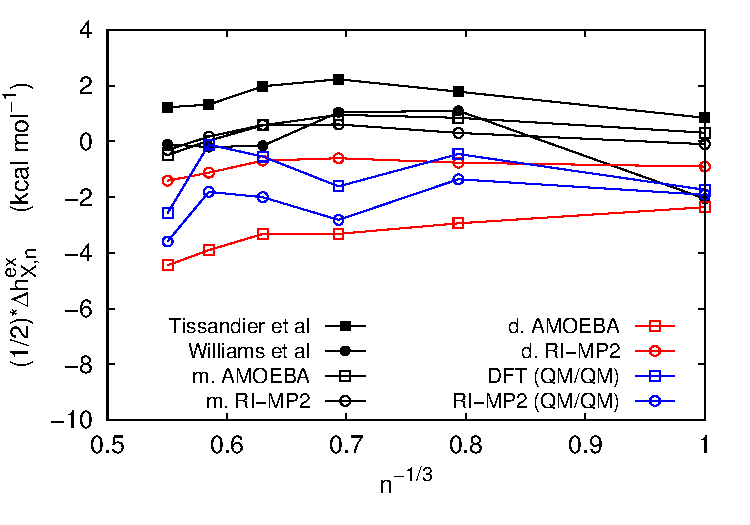
\includegraphics[width=0.98\linewidth]{images/cpa/deltaH_exptl_range-eps-converted-to.pdf}
 \end{center}
\caption[Half the enthalpy differences in the Na\sur{+}$\rightarrow$F\sur{-} transition for small clusters]{Half the difference in the enthalpy for the Na$^+$ to 
F$^-$ transition in the \emph{n} = 1--6 clusters. All simulations allowed free motion of the ions in the clusters. The plot labeled ``Tissandier'' (black solid squares) is 
for experimental data from Ref. \cite{coe1998cpa1}, and the plot labeled ``Williams'' (black solid circles ) is for experimental data from Ref.
\cite{donald2010expand_cpa} obtained from a larger range of experiments. ``m. AMOEBA'' (black open squares) refers to results from the modified AMOEBA model, while 
for ``m. RI-MP2'' the energies were computed at the MP2 level (with modified AMOEBA sampling). ``d. AMOEBA'' (red open squares) indicates the default AMOEBA model, 
and ``d. RI-MP2'' (red open circles) is for energies computed at the MP2 level (with default AMOEBA sampling). ``DFT(QM/QM)'' (blue open squares) labels the DFT
simulation results, and ``RI-MP2(QM/QM)'' (blue open circles) indicates DFT sampling with energy calculations at the MP2 level. The cluster size is displayed as 
n$^{-1/3}$.}
\label{fig:dHexptsmall}
\end{figure}

  To further explore the role of electronic quantum effects in the small clusters, I computed enthalpy differences for several other cases. First, I generated
  configurations with both the modified and default Thole parameter simulations, and computed the energies at the MP2 level. The MP2-computed enthalpy differences
  (using the modified Thole parameter for the sampling) accurately match the modified AMOEBA results. When the default Thole parameter is used to generate the
  configurations, the MP2 results lie between the default AMOEBA results and experiment. 
  
  Finally, configurations were also generated with B3LYP-D3/DFT simulations. When the energies are computed at the same level of theory, it is apparent the quantum
  model yields results more negative than experiment (except for the \emph{n} = 5 case). It is interesting that, when energies are computed at the MP2 level (with DFT
  configurations), larger deviations from experiment are observed. Nuclear quantum effects were not included in the DFT simulations, and based on the discussion 
  above these would likely move the computed values upward toward the experimental results. It is important to note the AMOEBA model was parametrized based on MP2 
  level calculations (with no inclusion of nuclear quantum effects)\cite{amoeba}. From the above results, I can conclude that the modified AMOEBA model
  for the F$^-$ ion yields quite accurate results for the energetics of the cation to anion transition in the small clusters. 

  Next I'll explore the size dependence of the cation-anion enthalpy difference over a large range of cluster sizes (up to \emph{n} = 200). As in Ref. \cite{pollard2014cpa1}, 
  I first constrain each ion to the cluster center of mass for clusters of \emph{n} $\geq$ 5. Figure \ref{fig:dHcom} displays the enthalpy difference as a function 
  of cluster size using the modified AMOEBA model and MP2 calculations. First, it is clear that a shift to more negative values develops as the cluster size is 
  increased beyond \emph{n} = 6. The shift appears to stabilize (with some oscillation) at a value of roughly $-4$ kcal/mol; already by the \emph{n} = 10 cluster size, 
  the majority of the shift has occurred. This is just beyond the scope of the myriad CPA studies\cite{coe1998cpa1,coe2001cpa2,coe2002cpa3,donald2010expand_cpa,kelly2006cpa}
  but still within the range of both experimental and theoretical used to generate the smaller cluster data\cite{wheeler2015hydration}.
  
\begin{figure}
 \begin{center}
  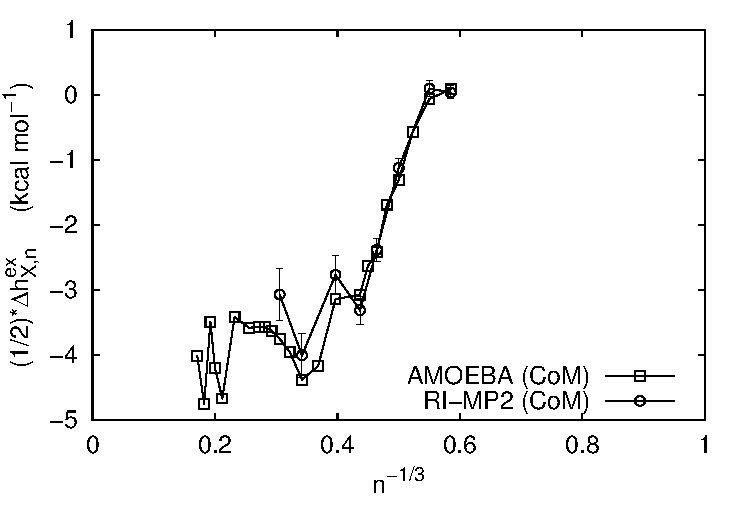
\includegraphics[width=0.98\linewidth]{images/cpa/deltaH_com-eps-converted-to.pdf}
 \end{center}
\caption[Half the enthalpy differences in the Na\sur{+}$\rightarrow$F\sur{-} transition for clusters with the ion fixed at the center of mass]{Half the difference 
in the enthalpy for the the Na$^+$ to F$^-$ transition in larger clusters (up to \emph{n} = 200). The energies were computed from modified (reduced Thole factor) AMOEBA
trajectories block-averaging every 100 steps for the case of the ion bound to the cluster center of mass (CoM). The results are compared out to \emph{n} = 35 with a sample 
of configurations modeled at the RI-MP2/aug-cc-pVDZ/aug-cc-pVDZ-RI level of theory. The cluster size is given as \emph{n}$^{-1/3}$. Error bars for AMOEBA averages are smaller
than the size of the symbols.}
\label{fig:dHcom}
\end{figure}

  In Ref. \cite{pollard2014cpa1} there was some discussion of the difficulties in obtaining converged enthalpy differences for the larger cluster sizes (involving the 
  difference of two large numbers and possible partial evaporation events). However, the previous free energy results (which are less affected by the difficulties in 
  the enthalpy calculations) fully support the notion that the net potential stabilizes for clusters in the size range considered here.  

  There is remarkable agreement of the MP2 results out to \emph{n} = 35 with the classical results. Since the configurations were generated with the modified AMOEBA model, 
  perhaps this is not so surprising; it does show that, for a given set of configurations, the model accurately mimics the energetics obtained from the realistic
  quantum electron distribution. The configurations are for the ions fully coupled to the nearby waters, and do not rely on a particular cavity definition.  

  The agreement of the modified AMOEBA results with experiments on small clusters discussed above then suggests this model is accurately representing the energetics
  over the full size range. It seems highly unlikely that errors in half the enthalpy difference of magnitude 10 kcal/mol occur (pushing the asymptotic values of the
  curves in Figures \ref{fig:dHcom} and \ref{fig:dHfree} downward by $\approx 10$ kcal/mol); such a shift magnitude would be necessary to produce a net potential 
  close to zero. 

  For the case in which the ions are free to move about the entire cluster, similar results are obtained (Figure \ref{fig:dHfree}). The enthalpy differences first
  stabilize at a slightly higher energy relative to Figure \ref{fig:dHcom}, but then relax to the asymptotic value of $-4$ kcal/mol. Again, the quantum results are 
  very close to the AMOEBA results.  The results show that locating the ion at the cluster center (aimed at more rapid convergence to the bulk limit) has only a 
  small effect on the computed results for this kosmotropic ion pair.  

\begin{figure}
 \begin{center}
  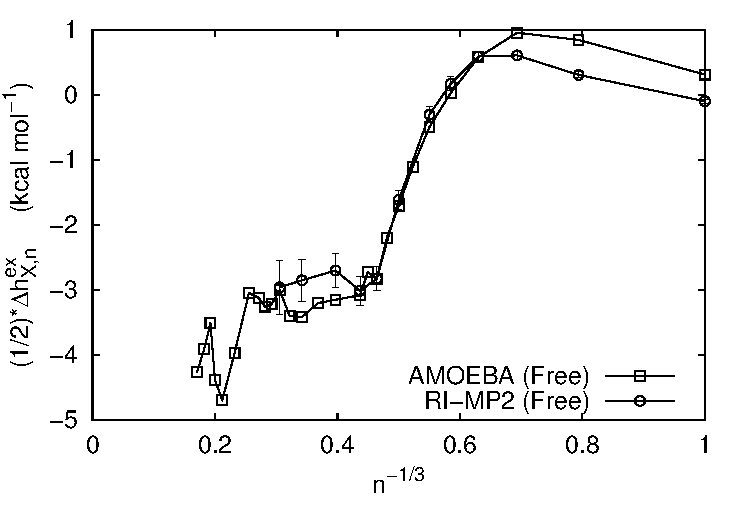
\includegraphics[width=0.98\linewidth]{images/cpa/deltaH_free-eps-converted-to.pdf}
 \end{center}
\caption[Half the enthalpy differences in the Na\sur{+}$\rightarrow$F\sur{-} transition for clusters with the ion unconstrained]{Half the difference in the enthalpy 
for the the Na$^+$ to F$^-$ transition in larger clusters (up to \emph{n} = 200). The energies were computed from modified (reduced Thole factor) AMOEBA trajectories
block-averaging every 100 steps for the case of the ion free to move throughout the cluster. The results are compared out to \emph{n} = 35 with a sample of configurations
modeled at the RI-MP2/aug-cc-pVDZ/aug-cc-pVDZ-RI level of theory. The cluster size is given as n$^{-1/3}$. Error bars for AMOEBA averages are smaller than the size of
the symbols.}
\label{fig:dHfree}
\end{figure}

  Considering the extension of these differences to the `gold standard' CCSD(T) method, I found similar agreement to that which I established earlier between AMOEBA
  and the MP2 method, see Figure \ref{fig:dHfreeall}. Out to a size of \emph{n} = 3, the quantum results fall more negative than the AMOEBA result at an intermediate
  energy to that predicted by Tissandier et al. and Williams et al. in Refs. \cite{coe1998cpa1} and \cite{donald2010expand_cpa}, respectively. Interestingly, there
  seems to be better overlap between the CCSD(T)/jun-cc-pVTZ and MP2 trends than when using CCSD(T)/aug-cc-pVDZ implying a fortuitous result at the lower level of 
  theory which is of similar quality to the much more prohibitive triple-$\zeta$ coupled-cluster method. Most importantly however, each of the trends tracks the drift
  in the Na\sur{+}/F\sur{-} pair enthalpy differences from near zero.

\begin{figure}
 \begin{center}
  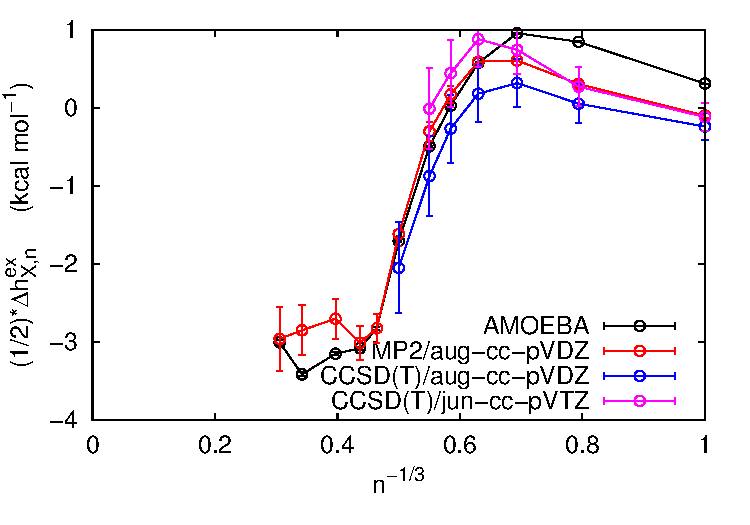
\includegraphics[width=0.98\linewidth]{images/cpa/deltaH_all-eps-converted-to.pdf}
 \end{center}
\caption[Half the enthalpy differences in the Na\sur{+}$\rightarrow$F\sur{-} transition at several levels of theory]{Half the enthalpy differences in the transition of 
Na $\rightarrow$ F, expressed in kcal/mol across varying theoretical treatments for clusters with up to \emph{n} = 35.}
\label{fig:dHfreeall}
\end{figure}

  A comparison between the AMOEBA and MP2 energies to the higher levels of theory revealed that the bulk of the figures fall within $\pm$ 0.5 kcal/mol of the higher 
  level estimate, see Figure \ref{fig:dHfreediffs}. The AMOEBA model tended to produce more positive energies than CCSD(T) except beyond \emph{n} = 3 for CCSD(T)/jun-cc-pVTZ, 
  while MP2 was slightly more negative than CCSD(T)/jun-cc-pVTZ and more positive than CCSD(T)/aug-cc-pVDZ. Differences between the AMOEBA and quantum methods tended to
  exhibit non-linear fluctuations while those between MP2 and CCSD(T) were approximately linear over the range considered. Overall, however, I find remarkable agreement
  between the methods.

\begin{figure}
 \begin{center}
  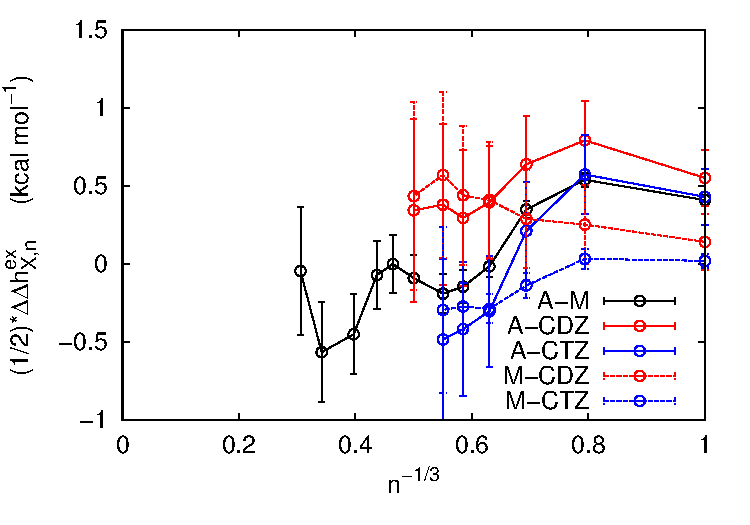
\includegraphics[width=0.98\linewidth]{images/cpa/deltaH_diffs_all-eps-converted-to.pdf}
 \end{center}
\caption[Differences in $\frac{1}{2}h\sursous{ex}{X,n}$ between methods]{Comparison of $\frac{1}{2}\Delta h\sursous{ex}{X,n}$ for the the Na$^+$ to F$^-$ transition, expressed
in kcal/mol between the various methods, 1) AMOEBA minus MP2/DZ, 2) AMOEBA minus CCSD(T)/DZ, 3) AMOEBA minus CCSD(T)/TZ, 4) MP2/DZ minus CCSD(T)/DZ, and 5) MP2/DZ minus
CCSD(T)/TZ. A is shorthand for AMOEBA, M for MP2, CDZ for CCSD(T)/DZ, and CTZ for CCSD(T)/TZ. DZ and TZ refer to aug-cc-pVDZ and jun-cc-pVTZ basis sets, respectively.}
\label{fig:dHfreediffs}
\end{figure}

  Projecting the MP2 to CCSD(T) errors to the bulk limit, assuming the \emph{n}$\sur{-\frac{1}{3}}$ dependence remains linear, it is clear that the errors in the reported
  enthalpy differences aren't likely to exceed 1 kcal/mol, see Figure \ref{fig:ccsdterror}. Granted, the trend approaches an asymptotic limit of about -4 kcal/mol at large 
  \emph{n}. However, even the AMOEBA to MP2 differences start off relatively linearly before oscillating in the range of $\pm$0.5 kcal/mol from zero. It's likely given that
  AMOEBA was parameterized against MP2 that the MP2 to CCSD(T) errors will also start to oscillate, making the linear projection a sort of \emph{worst case scenario}. Errors
  assuming the linear and oscillatory trends are discussed below.

\begin{figure}
 \begin{center}
  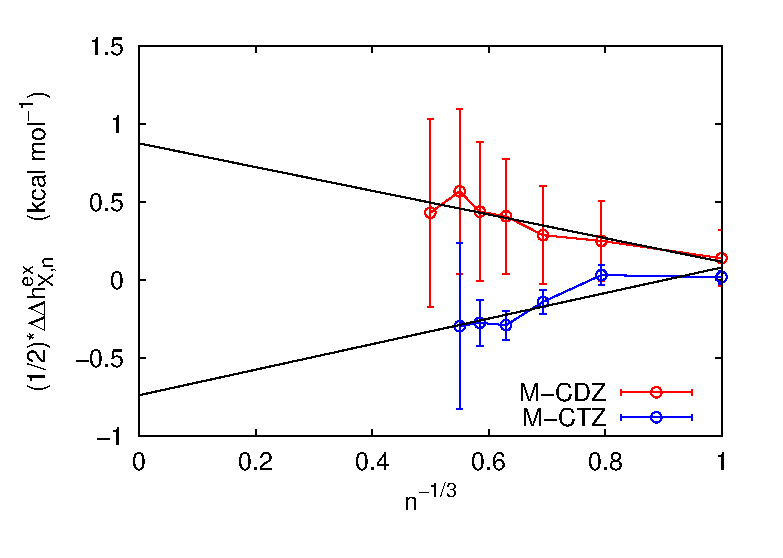
\includegraphics[width=0.98\linewidth]{images/cpa/deltaH_ccsdt_fit.eps}
 \end{center}
\caption[Estimated error in the MP2-level enthalpy relative to CCSD(T)]{Differences in $\frac{1}{2}\Delta h\sursous{ex}{X,n}$ (MP2 minus CCSD(T)) in the transition of Na 
$\rightarrow$ F, expressed in kcal/mol. Here M is shorthand for MP2, CDZ for CCSD(T)/aug-cc-pVDZ, and CTZ for CCSD(T)/jun-cc-pVTZ. The solid black lines are linear fits 
through the data and provide an estimate of the error in the enthalpy shift to large cluster size.}
\label{fig:ccsdterror}
\end{figure}

  Using Equation \ref{eq:netpot2}, I display in Figure \ref{fig:netpotsim} the size dependence of the derived net potential. As discussed above, I assume a
  temperature derivative of the net potential of zero. It is clear from the plot that the net potential approaches an asymptotic value of close to $-9.4$ kcal/mol-$e$
  discussed in Refs. \cite{beck2013sp} and \cite{pollard2014cpa1}. Compare this with the result assuming the -9.9 cal/mol-K-\emph{e} temperature derivative in Figure
  \ref{fig:netpotlps}. Given my discussion of the errors previously, it is instructive to note that the nearest alternative estimate of the electrochemical surface 
  potential is +3 kcal/mol-\emph{e} (+0.13 V). The linear estimate produces a 25\% error in my estimate of $\phi\sous{np}$ with a lower limit of $\approx~$-6.8 kcal/mol-\emph{e}. 
  Taking the oscillations of the AMOEBA to MP2 trend as an estimate of the error instead, I expect a more realistic uncertainty of -9.4 $\pm$ 1.1(25) kcal/mol-\emph{e} which
  is half the estimate of the \emph{worst case scenario} spelled out above. In volts that's -0.41 $\pm$ 0.05 V, though I always round down to -0.4 V.
  
\begin{figure}
 \begin{center}
  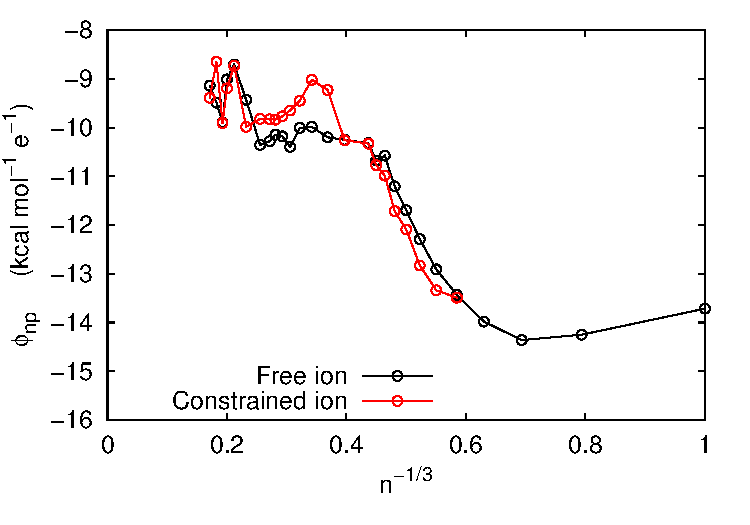
\includegraphics[width=0.98\linewidth]{images/cpa/net_pot_no_temp_deriv-eps-converted-to.pdf}
 \end{center}
\caption[Net potential with no temperature derivative]{The electrochemical surface potential as a function of cluster size up to \emph{n} = 200 (using Equation \ref{eq:netpot2}).
The temperature derivative ofthe net potential was assumed to be zero, as discussed in the text. The plots are for the cases in which the ions was either restricted to the
cluster center of mass or free to move throughout the cluster. The F$^{-}$ Thole damping parameter has been reduced from the default 0.39 value to 0.2 in generating the trajectories. 
The cluster size is given as n$^{-1/3}$. Error bars are comparable to or smaller than the size of the points (approximately $\pm$ 0.10 kcal mol$^{-1}$ or less).}
\label{fig:netpotsim}
\end{figure}

  The final result presented here is the size dependence of the net potential assuming the experimental temperature derivative to be reasonable\cite{randles1977structure} 
  as is asserted in Ref. \cite{hunenberger2011sp}. Interestingly this shifts the asymptote of the curve to around -11.6 kcal/mol-\emph{e} which is the average of the charge 
  dependent shifts in Ref. \cite{ashbaugh2008lps}. However, as has been noted by others\cite{donald2010expand_cpa,pollard2014cpa1}, this temperature derivative drives the
  proton solvation entropy much too negative. The CPA predicted proton solvation entropy is on the order of -30.3 to -33.5 cal/mol-K\cite{coe1998cpa1,donald2010expand_cpa}
  while bulk thermodynamic measurements predict a bulk solvation entropy of -24.7 cal/mol-K\cite{conway1978evaluation} using 0.878 mV/K for the temperature dependence of 
  the hydrogen electrode (from Ref. \cite{conway1993non}). This result is identical to that reported by Marcus\cite{marcus1985book}. Adding the negative surface potential 
  temperature derivative should push this quantity less negative to around -15 cal/mol-K. The corrected results from Ref. \cite{vlcek2013cpa} require a larger and negative
  temperature derivative and give a proton hydration entropy of only -5.3 cal/mol-K. This value cannot be recommended when the derivative is suspected of being very small.
  Note, these entropies reflect the 1 M ideal gas and 1 M solution standard state which adds a factor of 1900 cal/mol / 300 K to the literature values reported here. The 
  -1900 cal/mol is the free energy standard state correction and the entropy correction is the negative of the free energy correction divide the temperature.

\begin{figure}
 \begin{center}
  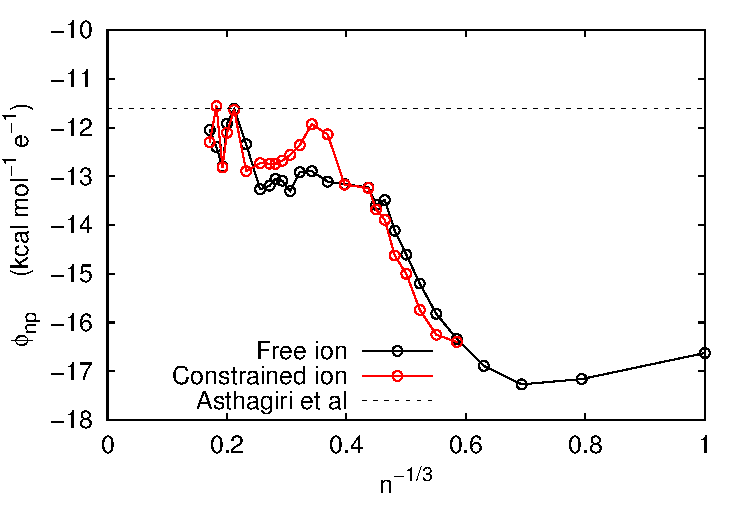
\includegraphics[width=0.98\linewidth]{images/cpa/net_pot-eps-converted-to.pdf}
 \end{center}
\caption[Net potential assuming experimental temperature derivative]{The electrochemical surface potential as a function of cluster size up to \emph{n} = 200 (using Equation 
\ref{eq:netpot2}). The temperature derivative of the net potential was assumed to be -9.9 cal/mol-K-\emph{e}, as taken from Randles\cite{randles1977structure}. The plots 
are for the cases in which the ions was either restricted to the cluster center of mass or free to move throughout the cluster. The F$^{-}$ Thole damping parameter has
been reduced from the default 0.39 value to 0.2 in generating the trajectories. The cluster size is given as n$^{-1/3}$. Error bars are comparable to or smaller than 
the size of the points (approximately $\pm$ 0.10 kcal mol$^{-1}$ or less). The dashed horizontal line is the -11.6 kcal/mol-\emph{e} value taken as an average of sign dependent
deviation in the LPS model of Ref. \cite{ashbaugh2008lps}.}
\label{fig:netpotlps}
\end{figure}

  \section{\label{ch5:sec4:level1}Discussion~}
  In conjunction with the results from Chapter \ref{ch5:sec3:level2}, my efforts suggest a proton hydration free energy of -264.7 kcal/mol, an enthalpy of -271.9 kcal/mol, an 
  entropy of -24 cal/mol-K, an electrochemical surface potential of water of -0.4 V, and a temperature derivative of the potential that is close to zero at room temperature. 
  These were revised in Ref. \cite{pollard2014cpa2} to a free energy of -264.2 kcal/mol, an enthalpy of -271.6 kcal/mol, an entropy of -24.5 cal/mol-K presented in the paper
  but not touched on here. In general, the values reported in Ref. \cite{pollard2014cpa2} should supersede those presented in Ref. \cite{pollard2014cpa1}.

  The above values differ in several respects from previous discussions and ongoing work. H\"{u}nenberger and Reif\cite{hunenberger2011sp} present an exhaustive compilation
  of proton hydration data, and based on an average of 98 values, recommend -264.8 kcal/mol for the free energy, -272.2 kcal/mol for the enthalpy, and -25 cal/mol-K for
  the entropy (labelled as \emph{intrinsic} or bulk values). While these results appear to agree well with the real values listed above, they are obtained as an
  average over data that includes both bulk and real quantities. The averaging then blurs the distinction drawn here between bulk and real quantities and its likely
  importance in determining the surface potential. The recommended real values in Ref. \cite{hunenberger2011sp} are -261.7 kcal/mol (free energy), -266.2 kcal/mol (enthalpy), 
  and -15.2 cal/mol-K, respectively, showing a large deviation from the results obtained here. 

  Ref. \cite{hunenberger2011sp} also recommends an electrochemical surface potential value of +0.13 V and a temperature derivative of -9.9 cal/mol-\emph{e} (-0.42 mV/K-\emph{e}). 
  The temperature derivative is similar to the result previously discussed by Randles\cite{randles1977structure}; from that temperature derivative, and an extrapolation to the
  critical point of water, Randles obtained a value for the electrochemical surface potential close to the +0.13 V value. Ref. \cite{hunenberger2011sp} discusses several possible
  concerns related to the previous experimental analysis of the temperature derivative. Also, it's worth mentioning that a smooth extrapolation from room temperature and 
  atmospheric pressure to the critical point is not likely a justified route for obtaining the net potential. 

  In a recent theoretical study aimed at examining the role of dispersion in ion solvation,\cite{duignan2013continuum2} the surface potential value recommended by H\"{u}nenberger
  and Reif\cite{hunenberger2011sp} was used, and it was argued that the CPA values such as those in Refs. \cite{coe1998cpa1} and \cite{donald2010expand_cpa} are bulk (or intrinsic)
  values that include no surface potential contribution. Previous simulations of large clusters, however, have been shown to include a surface potential 
  contribution\cite{beck2013sp,pollard2014cpa1}. The agreement of the computed (large cluster) results with the modified CPA analysis presented here (that is free of 
  extra-thermodynamic assumptions) provides clear evidence that the CPA-derived values correspond to the real quantities and not the bulk quantities. My results for the net
  potential rely on the assumption that the Marcus values are the bulk quantities, however. The main evidence in favor of this interpretation is the agreement between the 
  Marcus\cite{marcus1985book} and LPS\cite{ashbaugh2008lps} scales (after adjusting for the -11.6 kcal/mol potential).

  Finally, recent simulation studies of the electrostatic potential at the center of neutral cavities in water implies a value close to zero for the net 
  potential\cite{baer2012electrochemical,remsing2014lp}. In this work, the cavity was created by providing a repulsive force on the water oxygens. A previous study\cite{shi2013length} 
  showed, however, that the potential can change significantly if repulsions are included (in classical models) on the water hydrogens. An interesting alternative would be to 
  strictly enforce the cavity by excluding all electron density.

  \section{\label{ch5:sec5:level1}Conclusions~}
  The present chapter thus provides a contrasting view of proton hydration and the water surface potential. I have approached the problem from an alternative 
  thermodynamic direction that does not rely on direct electrostatic calculation of the net potential but rather infers its value by comparing ion enthalpy differences
  in large clusters with tabulated bulk values. Due to the relatively rapid convergence with cluster size of the enthalpy differences for the NaF kosmotropic pair (in
  the range \emph{n} = 10--20), it is hoped that experimental results on clusters in this size range may provide a test of the theoretical proposals outlined here.
  
  Additionally, this work has independently derived a single-ion thermodynamic scale when combined with the conventional (relative to H\sur{+}) thermodynamic scale.
  This scale defines real hydration properties which differ from the bulk values by inclusion of the net potential I reviewed previously. This scale differs somewhat 
  from the CPA scale of Tissandier et al.\cite{coe1998cpa1} and a separate recently derived scale of Vlcek et al.\cite{vlcek2013cpa} but is similar to that described 
  by Zhan et al.\cite{zhan2001absolute}. I would recommend that additional work to resolve the issues with the temperature derivative be performed. These calculations
  are planned using the Tinker package\cite{ponder2004tinker} and the iAMOEBA (improved AMOEBA) model which performs well for a number of properties over a broad 
  temperature and pressure range. A model equation of state will be useful in directing targeted simulations with greater accuracy with \emph{ab initio} molecular dynamics.

\end{cpa}